% =====================================================================
%  Chapitre 5 -- Projet de bout en bout, interprétabilité et éthique (3 h)
%  Introduction au Machine Learning -- CNFSDP -- L3 S5 -- 2026-2027
%  Version niveau licence (12/10/2026)
%  Compilation : pdflatex chapitre5.tex (deux fois)
%  Figures : code/figures_chapitre5.py (données fictives : code/enfants_dhs.py)
% =====================================================================
\documentclass[aspectratio=169,11pt]{beamer}
\usetheme{CNFSDP}
\usetikzlibrary{positioning,arrows.meta}
\usepackage{colortbl}

\chapitre{5}
\chapitrecourt{Ch.~5 \textendash{} De bout en bout}

\title{Chapitre 5 \textendash{} Projet de bout en bout, interprétabilité et éthique}
\subtitle{Des données d'enquête à un modèle que l'on peut expliquer et défendre}
\author{Rois Céti DIMBAMBA}
\institute{Ingénieur statisticien économiste \textperiodcentered{} Actuaire \textperiodcentered{} \href{https://rdimbamba.shinyapps.io/roisceti_e-cv/}{\textcolor{cnfVert}{CV en ligne}}}
\date{?? novembre 2026}

\begin{document}

% ---------------------------------------------------------------------
\begin{frame}[plain,noframenumbering]
  \titlepage
\end{frame}

\begin{frame}{Plan et objectifs}
  \begin{columns}[T]
    \begin{column}{0.44\textwidth}
      \footnotesize\tableofcontents
    \end{column}
    \begin{column}{0.54\textwidth}
      \begin{objectifs}
        \footnotesize
        \begin{itemize}
          \item Mener un projet complet : question, données d'enquête, préparation, modèles, évaluation.
          \item Construire un \emph{pipeline} et éviter les fuites d'information.
          \item Expliquer un modèle : importance des variables, dépendance partielle.
          \item Protéger les personnes enquêtées et vérifier l'équité d'un modèle.
          \item Lancer le projet de groupe sur l'EDS Congo.
        \end{itemize}
      \end{objectifs}
      \vskip-1mm{\scriptsize\color{cnfGris}Prérequis : chapitres~1 à~4.}
    \end{column}
  \end{columns}
\end{frame}

% =====================================================================
\section{La démarche d'un projet}

\begin{frame}{Sept étapes}
  \centering
  \begin{tikzpicture}[
      etape/.style={draw=cnfVert,fill=cnfVertPale,rounded corners=1.2mm,inner sep=1.4mm,text width=2.75cm,align=center,font=\footnotesize,minimum height=1.35cm},
      lien/.style={-{Stealth[length=1.6mm]},draw=cnfGris,semithick}]
    \node[etape] (e1) at (0,0) {\textbf{1. Question}\\que veut-on prédire, pour quelle décision ?};
    \node[etape] (e2) at (3.4,0) {\textbf{2. Données}\\lire, comprendre les codes et les variables};
    \node[etape] (e3) at (6.8,0) {\textbf{3. Préparation}\\manquants, codage, standardisation};
    \node[etape] (e4) at (10.2,0) {\textbf{4. Découpage}\\apprentissage et test, avant tout};
    \node[etape] (e5) at (10.2,-2.1) {\textbf{5. Modèles}\\comparer par validation croisée};
    \node[etape] (e6) at (6.8,-2.1) {\textbf{6. Évaluation}\\une fois sur le test, avec IC};
    \node[etape] (e7) at (3.4,-2.1) {\textbf{7. Interprétation}\\variables, équité, limites};
    \node[etape,draw=cnfJaune!70!black,fill=cnfJaune!12] (e8) at (0,-2.1) {\textbf{Communiquer}\\rapport, soutenance, code};
    \draw[lien] (e1) -- (e2); \draw[lien] (e2) -- (e3); \draw[lien] (e3) -- (e4); \draw[lien] (e4) -- (e5);
    \draw[lien] (e5) -- (e6); \draw[lien] (e6) -- (e7); \draw[lien] (e7) -- (e8);
  \end{tikzpicture}
  \vskip4mm
  \begin{exemple}[Fil rouge du chapitre]
    Prédire si un enfant de $12$ à $23$ mois a reçu toutes ses vaccinations, pour cibler les relances des agents de santé. Les données sont \emph{fictives} mais ont la forme du fichier « enfants » (KR) des enquêtes DHS : $3\,000$ enfants.
  \end{exemple}
\end{frame}

\begin{frame}{Poser la bonne question}
  \begin{itemize}
    \item \textbf{Quelle décision ?} Relancer les familles dont l'enfant risque de ne pas être vacciné. Le modèle sert à \emph{classer} les enfants par priorité.
    \item \textbf{Quelles variables sont disponibles au moment de la décision ?} Région, milieu, instruction de la mère, richesse, lieu d'accouchement, visites prénatales\dots{} mais pas le nombre de doses déjà reçues, qui définit la réponse.
    \item \textbf{Quelle erreur coûte le plus ?} Oublier un enfant non vacciné (faux négatif) plutôt qu'une relance inutile : on regardera le rappel (chapitre~1).
    \item \textbf{Prédire ou expliquer ?} Un bon prédicteur n'indique pas de causes : « la richesse prédit la vaccination » ne dit pas que distribuer de l'argent ferait vacciner.
  \end{itemize}
  \begin{aretenir}
    La question fixe la cible, les variables autorisées et la métrique. Elle se décide \emph{avant} de toucher aux données.
  \end{aretenir}
\end{frame}

% =====================================================================
\section{Lire et préparer des données d'enquête}

\begin{frame}{Les fichiers des enquêtes DHS}
  \begin{columns}[T]
    \begin{column}{0.5\textwidth}
      \small
      \begin{itemize}
        \item Un fichier par unité : ménages (\texttt{HR}), femmes (\texttt{IR}), hommes (\texttt{MR}), enfants (\texttt{KR})\dots
        \item Noms standard : \texttt{CGKR61FL.DTA} = Congo, enfants, enquête 6, Stata.
        \item Formats Stata (\texttt{.DTA}) et SPSS (\texttt{.SAV}) : chaque variable est un \emph{code} accompagné d'\emph{étiquettes}.
        \item Codes spéciaux : $98$ = « ne sait pas », $99$ = manquant ; à transformer en valeurs manquantes.
        \item Poids de sondage \texttt{v005} (à diviser par $10^6$) pour les statistiques descriptives.
      \end{itemize}
    \end{column}
    \begin{column}{0.46\textwidth}
      \small\centering
      \renewcommand{\arraystretch}{1.15}
      \begin{tabular}{ll}
        \toprule
        \textbf{variable} & \textbf{contenu} \\
        \midrule
        \texttt{v024}, \texttt{v025} & région, milieu \\
        \texttt{v106} & instruction de la mère \\
        \texttt{v190} & quintile de richesse \\
        \texttt{b4}, \texttt{bord} & sexe, rang de naissance \\
        \texttt{m14}, \texttt{m15} & visites prénatales, lieu \\
        \texttt{v467d} & distance au centre de santé \\
        \texttt{h2} à \texttt{h9} & vaccins reçus \\
        \bottomrule
      \end{tabular}
      \vskip1mm
      {\scriptsize\color{cnfGris}Toujours vérifier dans le dictionnaire de l'enquête.}
    \end{column}
  \end{columns}
\end{frame}

\begin{frame}{Préparer les variables}
  \begin{definition}[Codage en indicatrices (\emph{one-hot})]
    Une variable qualitative à $m$ modalités est remplacée par $m$ variables $0/1$, une par modalité. Exemple pour le lieu d'accouchement :
    \begin{center}
      \small\renewcommand{\arraystretch}{1.1}
      \begin{tabular}{lcccc}
        \toprule
        \texttt{m15} & domicile & hôpital public & clinique privée & autre \\
        \midrule
        hôpital public (21) & 0 & 1 & 0 & 0 \\
        domicile (11) & 1 & 0 & 0 & 0 \\
        \bottomrule
      \end{tabular}
    \end{center}
  \end{definition}
  \begin{definition}[Imputation, standardisation]
    \emph{Imputer}, c'est remplacer une valeur manquante, par exemple par la médiane de la variable.
    \emph{Standardiser}, c'est soustraire la moyenne et diviser par l'écart type (chapitres~2 à~4).
  \end{definition}
  {\small\color{cnfGris}Ne jamais utiliser un code comme $11$ ou $21$ comme un nombre : « clinique privée $(31)$ » n'est pas « trois fois domicile ».}
\end{frame}

\begin{frame}{Le pipeline : enchaîner sans tricher}
  \begin{definition}[Pipeline]
    Un \emph{pipeline} enchaîne la préparation et le modèle en un seul objet. Toutes les quantités de la préparation (médianes, moyennes, écarts types, modalités) sont apprises \emph{sur l'échantillon d'apprentissage seulement}, puis appliquées telles quelles au test.
  \end{definition}
  \centering
  \begin{tikzpicture}[
      boite/.style={draw=cnfVert,fill=cnfVertPale,rounded corners=1mm,inner sep=1.3mm,align=center,font=\footnotesize,text width=2.9cm,minimum height=1cm},
      lien/.style={-{Stealth[length=1.6mm]},draw=cnfGris,semithick}]
    \node[boite] (q) at (0,0.65) {variables qualitatives\\$\to$ indicatrices};
    \node[boite] (n) at (0,-0.65) {variables numériques\\$\to$ imputation, standardisation};
    \node[boite,text width=2.4cm] (m) at (4.2,0) {modèle\\logistique, forêt, boosting};
    \node[boite,text width=2.2cm,draw=cnfJaune!70!black,fill=cnfJaune!12] (p) at (7.6,0) {probabilité $\hat\eta(x)$};
    \draw[lien] (q.east) -- (m); \draw[lien] (n.east) -- (m); \draw[lien] (m) -- (p);
    \node[font=\scriptsize,color=cnfGris] at (0,1.55) {\texttt{ColumnTransformer}};
    \node[font=\scriptsize,color=cnfGris] at (4.2,1.0) {\texttt{Pipeline}};
  \end{tikzpicture}
  \vskip2mm
  \begin{flushleft}
    \small Avec un pipeline, la validation croisée refait toute la préparation dans chaque bloc : l'estimation de l'erreur reste honnête.
  \end{flushleft}
\end{frame}

\begin{frame}{Comparer trois modèles}
  \small
  Fil rouge : $2\,100$ enfants pour l'apprentissage, $900$ pour le test. Même pipeline de préparation, trois modèles, AUC par validation croisée à $5$ blocs :
  \begin{center}
    \renewcommand{\arraystretch}{1.25}
    \begin{tabular}{lcl}
      \toprule
      modèle & AUC (validation croisée) & commentaire \\
      \midrule
      régression logistique & $\mathbf{0{,}805}$ & simple, coefficients lisibles \\
      forêt aléatoire & $0{,}796$ & \\
      gradient boosting & $0{,}787$ & \\
      \bottomrule
    \end{tabular}
  \end{center}
  Sur le test, une seule fois : la logistique atteint une AUC de $0{,}824$ et une exactitude de $0{,}743$.
  \begin{remarque}[Lecture]
    Les écarts sont faibles. À performance voisine, on préfère le modèle le plus simple et le plus explicable : ici la logistique. Les méthodes d'ensemble gagnent quand les relations sont très non linéaires (chapitres~2 et~3).
  \end{remarque}
\end{frame}

% =====================================================================
\section{Les fuites d'information}

\begin{frame}{Qu'est-ce qu'une fuite ?}
  \begin{definition}[Fuite d'information]
    Il y a \emph{fuite} quand l'apprentissage utilise une information qui ne serait pas disponible au moment de prédire, ou qui vient de l'échantillon de test. L'erreur estimée devient trop optimiste.
  \end{definition}
  \textbf{Fuite n\textsuperscript{o}~1 : une variable qui contient la réponse.}
  \vskip1mm
  \small
  Le fichier contient \texttt{nb\_doses}, le nombre de doses reçues sur $8$. Or « vaccination complète » signifie justement \texttt{nb\_doses} $=8$.
  \begin{center}
    \renewcommand{\arraystretch}{1.2}
    \begin{tabular}{lc}
      \toprule
      variables utilisées & AUC (validation croisée) \\
      \midrule
      variables du fil rouge & $0{,}805$ \\
      les mêmes $+$ \texttt{nb\_doses} & $\mathbf{1{,}000}$ \\
      \bottomrule
    \end{tabular}
  \end{center}
  {\color{cnfGris}Un score parfait doit éveiller le soupçon : au moment de relancer une famille, on ne connaît pas encore ses doses.}
\end{frame}

\begin{frame}{Une fuite plus discrète : préparer avant de découper}
  \small
  \textbf{Fuite n\textsuperscript{o}~2.} $200$ individus, $2\,000$ variables de \emph{pur bruit}, une cible tirée à pile ou face : aucune méthode ne peut faire mieux que $50\,\%$ de bonnes réponses.
  \begin{center}
    \renewcommand{\arraystretch}{1.25}
    \begin{tabular}{p{0.62\textwidth}c}
      \toprule
      procédure & exactitude estimée \\
      \midrule
      on choisit les $20$ variables les plus liées à $y$ sur \emph{toutes} les données, puis validation croisée & $0{,}755$ \\
      le choix des $20$ variables est fait \emph{dans} le pipeline, bloc par bloc & $0{,}555$ \\
      \bottomrule
    \end{tabular}
  \end{center}
  La première procédure a « vu » les blocs de validation en choisissant les variables : elle annonce $75\,\%$ de réussite sur du hasard.
  \begin{aretenir}
    Règles : découper d'abord ; toute étape apprise sur les données (sélection, imputation, standardisation, choix de réglages) va dans le pipeline ; le test ne sert qu'une fois.
  \end{aretenir}
\end{frame}

% =====================================================================
\section{Interpréter un modèle}

\begin{frame}{Deux outils d'interprétation}
  \begin{definition}[Importance par permutation]
    Pour la variable $x_j$ : on mélange au hasard sa colonne dans les données test, ce qui casse son lien avec $y$, et l'on mesure la baisse de performance (ici de l'AUC). On répète plusieurs fois et l'on fait la moyenne.
  \end{definition}
  \begin{definition}[Dépendance partielle]
    Pour une valeur $v$ de la variable $x_j$ : on impose $x_j=v$ à \emph{tous} les individus, sans changer leurs autres variables, et l'on calcule la probabilité moyenne prédite. La courbe obtenue en faisant varier $v$ montre l'effet moyen de $x_j$ dans le modèle.
  \end{definition}
  {\small\color{cnfGris}Ces deux outils marchent pour n'importe quel modèle : logistique, forêt, boosting.}
\end{frame}

\begin{frame}{Ce que dit le modèle du fil rouge}
  \centering
  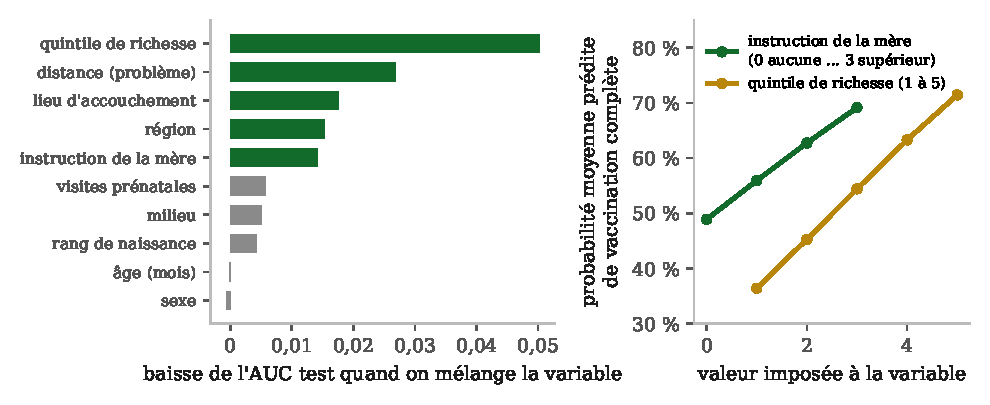
\includegraphics[width=0.75\textwidth]{interpretation.pdf}
  \vskip1mm
  \begin{minipage}{0.92\textwidth}
    \small
    Le quintile de richesse, la distance au centre de santé et le lieu d'accouchement sont les variables les plus utiles. Le sexe et l'âge de l'enfant n'apportent rien.
    En passant d'une mère sans instruction à une mère du supérieur, la probabilité moyenne prédite passe de $49$ à $69\,\%$.
  \end{minipage}
  \vskip1mm
  {\small\color{cnfGris}Précautions : ce sont des \emph{associations} ; deux variables corrélées (instruction et richesse) se partagent l'importance.}
\end{frame}

% =====================================================================
\section{Confidentialité}

\begin{frame}{Protéger les personnes enquêtées}
  \begin{columns}[T]
    \begin{column}{0.52\textwidth}
      \small
      \textbf{Retirer les noms ne suffit pas.} Des variables anodines, croisées, désignent une personne : ce sont des \emph{quasi-identifiants}.
      \vskip1mm
      Fil rouge : en croisant région, milieu, sexe, âge en mois, rang de naissance et instruction de la mère, \textbf{$37\,\%$ des enfants} sont seuls dans leur case, et $86\,\%$ sont dans une case d'au plus $3$ enfants.
      \vskip1mm
      Un voisin qui connaît ces six informations retrouverait la ligne de l'enfant, et donc ses réponses de santé.
    \end{column}
    \begin{column}{0.44\textwidth}
      \begin{aretenir}
        Conditions d'usage des données DHS :
        \begin{itemize}\setlength\itemsep{1pt}
          \item usage limité au projet déclaré ;
          \item fichiers reçus de l'enseignant, jamais retransmis, même dans un groupe ;
          \item aucune tentative d'identifier une personne ou un ménage ;
          \item fichiers jamais déposés sur GitHub ni envoyés par courriel.
        \end{itemize}
      \end{aretenir}
    \end{column}
  \end{columns}
\end{frame}

\begin{frame}{Publier un chiffre sans trahir personne}
  \begin{definition}[Mécanisme de Laplace]
    Pour publier un comptage $N$ (par exemple le nombre d'enfants non vaccinés d'un district), on publie $N+B$, où le bruit $B$ suit une loi de Laplace de paramètre $\frac1\varepsilon$ : moyenne $0$, écart type $\frac{\sqrt2}\varepsilon$.
  \end{definition}
  \begin{columns}[c]
    \begin{column}{0.52\textwidth}
      \begin{proposition}[admise]
        Ajouter ou retirer une personne change $N$ d'au plus $1$. Avec ce bruit, la loi du chiffre publié change alors d'un facteur au plus $e^\varepsilon$ : c'est la \emph{confidentialité différentielle} de niveau $\varepsilon$.
      \end{proposition}
      \small Petit $\varepsilon$ : forte protection, chiffre moins précis.
    \end{column}
    \begin{column}{0.46\textwidth}
      \centering
      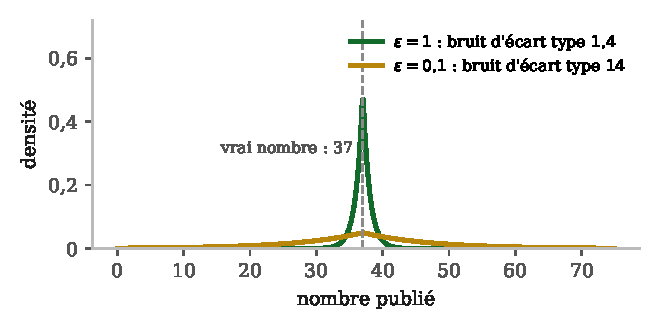
\includegraphics[width=\textwidth]{laplace.pdf}
    \end{column}
  \end{columns}
  \vskip1mm
  {\small\color{cnfGris}Le recensement des États-Unis de 2020 a été publié ainsi. L'arbitrage entre précision et protection est un choix public.}
\end{frame}

% =====================================================================
\section{Équité}

\begin{frame}{Un modèle peut-il être injuste ?}
  \small
  Le modèle signale les enfants à relancer (prédit « non vacciné »). Sur les $900$ enfants test, selon le milieu :
  \begin{center}
    \renewcommand{\arraystretch}{1.2}
    \begin{tabular}{lcccccc}
      \toprule
      milieu & enfants & non vaccinés & VP & FN & FP & VN \\
      \midrule
      urbain & $400$ & $79$ & $21$ & $58$ & $10$ & $311$ \\
      rural & $500$ & $303$ & $234$ & $69$ & $94$ & $103$ \\
      \bottomrule
    \end{tabular}
  \end{center}
  \begin{columns}[c]
    \begin{column}{0.48\textwidth}
      \begin{definition}[Trois critères d'équité]
        Entre deux groupes, on compare :
        \begin{itemize}\setlength\itemsep{1pt}
          \item la part d'individus signalés (\emph{parité}) ;
          \item le rappel (\emph{égalité des chances}) ;
          \item la précision (\emph{calibration}).
        \end{itemize}
      \end{definition}
    \end{column}
    \begin{column}{0.5\textwidth}
      \centering
      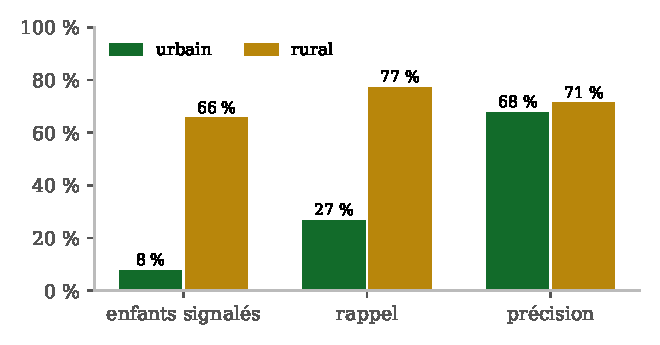
\includegraphics[width=0.94\textwidth]{equite.pdf}
    \end{column}
  \end{columns}
\end{frame}

\begin{frame}{Lire l'audit d'équité}
  \begin{itemize}\small\setlength\itemsep{1pt}
    \item \textbf{Précision voisine} ($68$ et $71\,\%$) : un enfant signalé l'est à raison aussi souvent en ville qu'à la campagne.
    \item \textbf{Rappel très différent} : $77\,\%$ des enfants ruraux non vaccinés sont repérés, mais $27\,\%$ seulement des urbains ($21$ sur $79$) : en ville, ils ressemblent aux vaccinés.
    \item \textbf{Signalements} : $66\,\%$ en milieu rural, $8\,\%$ en ville, car les taux de vaccination diffèrent vraiment.
  \end{itemize}
  \begin{proposition}[admise]
    Si la part de positifs diffère entre deux groupes, un classifieur imparfait ne peut pas égaliser à la fois précision, rappel et taux de faux positifs.
  \end{proposition}
  \begin{aretenir}
    On choisit le critère selon l'usage. Pour une campagne de vaccination, oublier un enfant est grave : on vise des rappels égaux (par exemple un seuil par milieu), et on l'écrit dans le rapport.
  \end{aretenir}
\end{frame}

% =====================================================================
\section{Le projet de groupe}

\begin{frame}{Le projet : organisation et livrables}
  \begin{columns}[T]
    \begin{column}{0.52\textwidth}
      \small
      \textbf{Groupes} : $36$ étudiants, $9$ groupes de $4$, une variante différente par groupe.
      \vskip1mm
      \textbf{Données} : EDS Congo 2011-2012 (DHS), fichiers originaux.
      \vskip1mm
      \textbf{Sujet} : sur la variante du groupe,
      \begin{itemize}\setlength\itemsep{1pt}
        \item une question de \emph{prédiction} (chapitres~1 à~3), modèles comparés par validation croisée ;
        \item une analyse \emph{non supervisée} (chapitre~4) : ACP, typologie ;
        \item un audit d'équité et une discussion des limites (chapitre~5).
      \end{itemize}
    \end{column}
    \begin{column}{0.44\textwidth}
      \small
      \renewcommand{\arraystretch}{1.25}\setlength\tabcolsep{4pt}
      \begin{tabular}{lr}
        \toprule
        \textbf{Évaluation du cours} & \textbf{poids} \\
        \midrule
        examen sur table (3 h) & $40\,\%$ \\
        rapport de $10$ pages + notebook & $40\,\%$ \\
        soutenance de $15$ min & $20\,\%$ \\
        \bottomrule
      \end{tabular}
      \vskip2mm
      \textbf{Calendrier} : remise du rapport et soutenances \textbf{fin novembre 2026}, deux à trois semaines après ce chapitre (dates exactes en salle).
      \vskip1mm
      {\footnotesize\color{cnfGris}À la soutenance, chacun des quatre membres présente une partie.}
    \end{column}
  \end{columns}
\end{frame}

\begin{frame}{Neuf groupes, neuf variantes}
  \footnotesize
  \renewcommand{\arraystretch}{1.1}\setlength\tabcolsep{4pt}
  \begin{tabular}{cllp{0.37\textwidth}p{0.3\textwidth}}
    \toprule
    \textbf{gr.} & \textbf{thème} & \textbf{fichier} & \textbf{cible à prédire} & \textbf{variante} \\
    \midrule
    1 & richesse & \texttt{HR} & ménage dans les 40 \% les plus pauvres & indice national (ACP), comparé à \texttt{hv271} \\
    2 & richesse & \texttt{HR} & ménage dans les 40 \% les plus pauvres & indices urbain et rural séparés \\
    3 & vaccination & \texttt{KR} & vaccination complète (\texttt{h2} à \texttt{h9}) & enfants de $12$ à $23$ mois \\
    4 & vaccination & \texttt{KR} & abandon : DTC1 reçu, DTC3 non & enfants de $12$ à $23$ mois \\
    5 & vaccination & \texttt{KR} & rougeole (\texttt{h9}) & enfants de $12$ à $23$ mois \\
    6 & nutrition & \texttt{KR} & retard de croissance (\texttt{hw70} $<-200$) & enfants de moins de $5$ ans \\
    7 & nutrition & \texttt{KR} & insuffisance pondérale (\texttt{hw71} $<-200$) & enfants de moins de $5$ ans \\
    8 & femme & \texttt{IR} & contraception moderne (\texttt{v313} $=3$) & femmes en union \\
    9 & femme & \texttt{IR} & besoins non satisfaits en contraception & femmes en union \\
    \bottomrule
  \end{tabular}
  \vskip2mm
  {\footnotesize\color{cnfGris}Attribution en salle. Codes à vérifier dans le dictionnaire (exclure les codes $\ge9996$ de \texttt{hw70}, \texttt{hw71}). Groupes 1 et 2 : prédire la pauvreté avec des variables hors indice (taille du ménage, chef de ménage, région).}
\end{frame}

\begin{frame}{Obtenir les données DHS}
  \begin{enumerate}
    \item L'enseignant a demandé au programme DHS une \textbf{autorisation pour toute la classe} : pas de compte à créer pour les étudiants.
    \item Chaque étudiant signe la \textbf{charte d'utilisation} du \emph{Guide du projet}.
    \item L'enseignant remet les fichiers (Stata ou SPSS : \texttt{HR}, \texttt{IR}, \texttt{KR}) et le dictionnaire des variables, par un canal privé.
    \item Chacun range les fichiers dans un dossier \texttt{donnees/} déclaré dans \texttt{.gitignore}.
    \item À la fin du cours, on supprime ses copies.
  \end{enumerate}
  \begin{aretenir}
    Ce qui est rendu : le code et le rapport, jamais les données. Aucun fichier DHS n'est retransmis : ni dans le groupe, ni entre groupes, ni sur Internet.
  \end{aretenir}
  {\small\color{cnfGris}Pour un mémoire ou une recherche après le cours, la demande se fait en son nom : procédure dans le \emph{Guide du projet}.}
\end{frame}

% =====================================================================
\section{En Python}

\begin{frame}[fragile]{Lire un fichier DHS avec pandas}
\begin{python}[basicstyle=\ttfamily\scriptsize]
import numpy as np, pandas as pd
fichier = "donnees/ZZKR_FICTIF.DTA"                   # sur l'EDS Congo : CGKR61FL.DTA
with pd.io.stata.StataReader(fichier) as lecteur:
    etiquettes = lecteur.value_labels()               # codes -> libellés
    libelles = lecteur.variable_labels()              # nom long de chaque variable
print(libelles["v106"], etiquettes["v106"])
colonnes = ["v024", "v025", "v106", "v190", "b4", "bord", "hw1", "m14", "m15", "v467d",
            "vacc_complet"]
df = pd.read_stata(fichier, columns=colonnes, convert_categoricals=False)
df["m14"] = df["m14"].replace(98, np.nan)             # 98 = « ne sait pas » -> manquant
print(df.shape, round(df["vacc_complet"].mean(), 3), df["m14"].isna().sum())
spss = pd.read_spss("donnees/ZZKR_FICTIF.SAV", usecols=colonnes)   # version SPSS (pyreadstat)
# niveau d'instruction de la mère {0: 'aucune', 1: 'primaire', 2: 'secondaire', ...}
# (3000, 11) 0.575 197
\end{python}
\vskip-1mm
{\small\color{cnfGris}\texttt{columns} ne charge que les variables utiles (les vrais fichiers en ont plus de mille) ; \texttt{convert\_categoricals=False} garde les codes, plus sûrs à manipuler.}
\end{frame}

\begin{frame}[fragile]{Préparer dans un pipeline}
\begin{python}[basicstyle=\ttfamily\scriptsize]
from sklearn.model_selection import train_test_split, cross_val_score
from sklearn.pipeline import make_pipeline
from sklearn.compose import make_column_transformer
from sklearn.preprocessing import OneHotEncoder, StandardScaler
from sklearn.impute import SimpleImputer

qual = ["v024", "v025", "b4", "m15", "v467d"]          # qualitatives
quant = ["v106", "v190", "bord", "hw1", "m14"]          # numériques
df[quant] = df[quant].astype(float)
X, y = df[qual + quant], df["vacc_complet"]
Xa, Xt, ya, yt = train_test_split(X, y, test_size=0.3, random_state=0, stratify=y)
prep = make_column_transformer(
    (OneHotEncoder(handle_unknown="ignore"), qual),                       # indicatrices
    (make_pipeline(SimpleImputer(strategy="median"), StandardScaler()), quant))
\end{python}
\vskip-1mm
{\small\color{cnfGris}On découpe d'abord ; \texttt{prep} n'apprend ses médianes, moyennes et modalités qu'au moment du \texttt{fit}, sur l'apprentissage.}
\end{frame}

\begin{frame}[fragile]{Comparer les modèles par validation croisée}
\begin{python}[basicstyle=\ttfamily\scriptsize]
from sklearn.linear_model import LogisticRegression
from sklearn.ensemble import RandomForestClassifier, GradientBoostingClassifier

modeles = {"logistique": LogisticRegression(max_iter=1000),
           "forêt": RandomForestClassifier(n_estimators=300, min_samples_leaf=10,
                                           random_state=0),
           "boosting": GradientBoostingClassifier(random_state=0)}
for nom, m in modeles.items():
    auc = cross_val_score(make_pipeline(prep, m), Xa, ya, cv=5, scoring="roc_auc")
    print(nom, auc.mean().round(3))
# logistique 0.805 | forêt 0.796 | boosting 0.787
\end{python}
\vskip-1mm
{\small\color{cnfGris}\texttt{make\_pipeline(prep, m)} : la préparation est refaite dans chaque bloc de la validation croisée, sans fuite.}
\end{frame}

\begin{frame}[fragile]{Importance des variables et audit d'équité}
\begin{python}[basicstyle=\ttfamily\scriptsize]
from sklearn.inspection import permutation_importance
f = make_pipeline(prep, LogisticRegression(max_iter=1000)).fit(Xa, ya)
r = permutation_importance(f, Xt, yt, scoring="roc_auc", n_repeats=20, random_state=0)
print(pd.Series(r.importances_mean, index=X.columns).nlargest(3).round(3).to_dict())
# {'v190': 0.05, 'v467d': 0.027, 'm15': 0.018}

# signalé = prédit « non vacciné »
signale = pd.Series(f.predict_proba(Xt)[:, 1] < 0.5, index=Xt.index)
non_vacc = yt == 0
for g, milieu in [(1, "urbain"), (2, "rural")]:
    m = Xt["v025"] == g
    print(milieu, round(signale[m].mean(), 2),          # part d'enfants signalés
          round(signale[m & non_vacc].mean(), 2),        # rappel
          round(non_vacc[m & signale].mean(), 2))        # précision
# urbain 0.08 0.27 0.68 | rural 0.66 0.77 0.71
\end{python}
\vskip-1mm
{\small\color{cnfGris}Un audit d'équité ne demande que quelques lignes : il fait partie de tout rapport de projet.}
\end{frame}

% =====================================================================
\section{TP en salle}

\begin{frame}{TP5 \textendash{} Un projet de bout en bout}
  \footnotesize
  \begin{tp}{TP5 \textendash{} à faire en salle}{45 min \textperiodcentered{} \texttt{notebooks/TP5.ipynb} (Colab)}
    \begin{enumerate}\setlength\itemsep{0pt}
      \item \textbf{Lecture} : fabriquer le fichier fictif au format DHS (Stata et SPSS), le relire avec pandas, lire les étiquettes, recoder $98$ en manquant.
      \item \textbf{Pipeline} : comparer logistique, forêt et boosting par validation croisée ; évaluer le meilleur une fois sur le test.
      \item \textbf{Fuites} : ajouter \texttt{nb\_doses} ; refaire l'expérience des $2\,000$ variables de bruit, sélection hors puis dans le pipeline.
      \item \textbf{Interprétation} : importance par permutation et dépendance partielle de l'instruction de la mère.
      \item \textbf{Confidentialité} : part d'enfants uniques sur six quasi-identifiants ; publier un comptage avec le mécanisme de Laplace pour $\varepsilon=1$ et $0{,}1$.
      \item \textbf{Équité} : audit par milieu ; chercher un seuil rural et un seuil urbain qui donnent le même rappel.
    \end{enumerate}
  \end{tp}
\end{frame}

\begin{frame}{Résumé}
  \begin{itemize}\small
    \item Un projet commence par une question : décision, variables disponibles au moment de prédire, métrique.
    \item Données d'enquête : codes et étiquettes, codes spéciaux, poids ; on ne lit que les variables utiles.
    \item Préparation (indicatrices, imputation, standardisation) et modèle dans un même pipeline ; on découpe d'abord.
    \item Fuites : variable qui contient la réponse, préparation faite avant le découpage. Un score trop beau est suspect.
    \item Interprétation : importance par permutation, dépendance partielle ; associations, pas causes.
    \item Confidentialité : quasi-identifiants, conditions d'usage DHS, bruit de Laplace.
    \item Équité : comparer signalements, rappels et précisions entre groupes ; choisir le critère selon l'usage.
  \end{itemize}
\end{frame}

\begin{frame}{Ce que vous savez faire à la fin du cours}
  \small
  \renewcommand{\arraystretch}{1.3}
  \begin{tabular}{p{0.2\textwidth}p{0.72\textwidth}}
    \toprule
    \textbf{Chapitre} & \textbf{Savoir-faire} \\
    \midrule
    1. Fondements & poser un problème d'apprentissage, mesurer une erreur, valider honnêtement \\
    2. Régression & moindres carrés, Ridge et Lasso ; forêt et boosting en régression \\
    3. Classification & $k$-NN, logistique, arbres ; bagging, forêts, AdaBoost, gradient boosting \\
    4. Non supervisé & ACP et indice de richesse ; k-means, CAH ; observations atypiques \\
    5. De bout en bout & pipeline sans fuite, interprétation, confidentialité, équité \\
    \bottomrule
  \end{tabular}
  \vskip3mm
  {\color{cnfGris}Pour aller plus loin : réseaux de neurones, SVM, théorie de la généralisation\dots{} dans un cours de machine learning approfondi. Questions : par message privé ou dans l'onglet Discussions du dépôt \texttt{\cnfDepot}.}
\end{frame}

\end{document}
